\ifx\allfiles\undefined
\documentclass[12pt, a4paper, oneside]{ctexbook}
%\usepackage{microtype}
\usepackage{amsmath, esint,amsthm, amssymb, bm, color, framed, graphicx, imakeidx, geometry,
hyperref, mathrsfs,lipsum,fancyhdr,indentfirst,array,tabularx,float,prettyref,stmaryrd}
%文内引用
%插入书签:\label{myref:引用内容(英文字母,中文出现了编译错误)}
%引用书签:\prettyref{myref:引用内容}

\allowdisplaybreaks[4]

%简化的指令
%\renewcommand{\i}{\mathrm{i}}%虚数i
\newcommand{\di }{\text{d}}%微分
\newcommand{\pian }{\partial}%偏导数
\newcommand{\die }{\textbf{d}}%外微分
\newcommand{\fuyi }{^{-1}}%逆映射
\newcommand{\card }{\text{card}}%势
\newcommand{\R }{\mathbb{R}}%实数
\newcommand{\Z }{\mathbb{Z}}%整数
\newcommand{\RR }{$\R\ $}%实数(文本)
\newcommand{\Rn }{$\R^n\ $}%实数(文本)
\newcommand{\N }{\mathbb{N}}%自然数
\renewcommand{\S}{\mathcal{S}}%S
\newcommand{\fai }{\varphi}%常用的那个小phi
\newcommand{\e }{\vec{e}}%向量e
\newcommand{\Id }{\text{Id}}%单位元
\newcommand{\continue }{\text{连续}}%连续
\newcommand{\C }{\mathcal{C}}%连续函数类
\newcommand{\Com }{\mathbb{C}}%复数
\newcommand{\M }{\mathcal{M}}%矩阵
\newcommand{\Hess }{\text{Hess}}%Hess矩阵
\newcommand{\normmm}[1]{{\left\vert\kern-0.25ex\left\vert\kern-0.25ex\left\vert #1 
   \right\vert\kern-0.25ex\right\vert\kern-0.25ex\right\vert}}%|||v|||三个竖线的范数
%常用的文本里的字母
\newcommand{\x }{$x$}\newcommand{\xo }{$x_0$}
\newcommand{\y }{$y$}\newcommand{\yo }{$y_0$}
\newcommand{\z }{$z$}\newcommand{\zo }{$z_0$}
\newcommand{\n }{$n$}\newcommand{\f  }{$ f $}

\title{
\vspace{-2cm}
  \begin{figure}[!t]%插入题目的图片
    \centering
    
\includegraphics[width=14cm]{shulijichu-2.png}
  \end{figure}
  \vspace{-2cm}
  {\Huge{\textbf{工程师学院数学理论基础\\
Fondements des Théories Mathématiques de l'Ecole d'Ingénieur de Chimie Pékin\\
第二部分:数学分析里的空间\\
Partie II: Espaces dans l'Analyse
}}}
}
\author{Augustin}
\date{最后更新于:\today}
\linespread{1.5}
\makeindex

\setcounter{tocdepth}{1}%两个2说明只显示到subsection
\setcounter{secnumdepth}{2}

%\def\allfiles{}
\begin{document}
\newrefformat{myref}{第\ref{#1} 节}
\vspace{-3cm}
\maketitle
\tableofcontents
\else
\part{数学分析里的空间\\ Espaces dans l'Analyse}
\fi
%开始本部分正文

\chapter{数列与数项级数\\Suites et Séries}

\chapter{$\R$上的一元函数\\ Fonctions d'Une Variable Réelle}

\chapter{Riemann积分\\ Intégrale de Riemann}

\chapter{函数列与函数项级数\\Suites et Séries de Fonctions}
  本章所研究的两个概念都是由以前学习过的数列(suite)和级数(série)推广而来.
  其中,函数列是数列的推广,函数项级数是数项级数的推广,二者都是以数列和级数的理论为基础建立.
  研究函数列和函数项级数,是为了用一种全新的方法定义函数,并讨论函数的性质,特别是收敛性(convergence)和连续性(continuité).
  基于此,我们可以研究算子的换序问题.

\section{函数列与函数项级数}
  \subsection{Définition}
  函数列指各项为具有相同定义域的函数的序列.
  I是$\R$上的区间,$\mathcal{F}(I)$是区间I上所有函数的集合.
  对一个有序列${f_n}\in\mathcal{F}(I)$,称${f_n}$为一个函数列.
  后续会一直默认${f_n}\in\mathcal{F}(I)$这个条件.\\

  函数项级数可以被简单地理解为函数列的加和.
  对于一个函数列${f_n}$,其函数项级数为$S_p=\sum_{n=0}^{p} f_n$,其中$p\in\mathbb{N}$.\\
  \subsection{Remarque:二者的关系}
  函数项级数和函数列有着密切的关系,正如数列和数项级数那样,
  一个函数项级数可以认为是某个函数列的构成的数列的前\n 项和,
  而函数列${f_n}$可以认为是函数项级数$S_p=\sum_{n=1}^{p} f_n-f_{n-1}$, $p\in\mathbb{N}, f_0=0$的\n 次部分和.
  因此函数列以及函数项级数的性质可以等价,我们只需要研究其中一个,自然就可以得到两个的结论.


\section{逐点收敛 Convergence simple}
  逐点收敛是函数列最基本的收敛,可以直观地理解为函数列${f_n}$里每个函数$f_i$定义域中,每个点$x$组成的数列${x}_n$随n都是收敛的.
  \subsection{Définition}
  逐点收敛的一种定义为:
  \begin{equation}
    \notag
    \forall x\in I, f_n(x)\xrightarrow[n\rightarrow\infty]{}f(x)
  \end{equation}
  此时称函数列$f_n(x)$在区间$I$上逐点收敛于$f(x)$ (La suite $f_n(x)$ convergence simplement vers $f(x)$ sur $I$).\\
  同理,对于函数项级数:
  \begin{equation}
    \notag
    \forall x\in I, \sum_{n=0}^{p} u_n(x)\xrightarrow[n\rightarrow\infty]{}U(x)
  \end{equation}
  称函数项级数$u_n(x)$在区间$I$上逐点收敛于$U(x)$.
  
  
  \subsection{Proposition:逐点收敛的算子交换}
  本章所研究的主要是针对于极限算子、Riemann积分算子和求导算子的交换问题.
  显然,对于逐点收敛这么弱的结论,三种算子都是不可交换的.\\
  \subsubsection{极限算子}
  设$I=[0,1] , f_n(x)=x^n$.显然$f_n$在区间$I$上有逐点收敛
  \begin{equation}
    \notag
    f_n\xrightarrow[n\rightarrow\infty]{}f=
    \begin{cases}
    0 &x\in[0,1)\\
    1 &x=1
    \end{cases}
  \end{equation}
  \begin{equation}
    \notag
    \lim_{n \to \infty} \lim_{x \to 1} x^n=1 \mbox{,然而由于$f$在1处不连续,} 
    \lim_{x \to 1}\lim_{n \to \infty} x^n \mbox{不存在}
  \end{equation}
  故极限算子无法交换.
  \subsubsection{求导算子}
  同上,$f$在1处不连续,故不可导,故求导算子无法交换.
  \subsubsection{Riemann积分算子}
  设$I=[0,1] , s_n(x)=2n^2xe^{-n^2x^2}$.显然$f_n$在区间$I$上逐点收敛于$s(x)=0$
  \begin{equation}
    \notag
    \lim_{n \to \infty} \int_{0}^{1}  2n^2xe^{-n^2x^2}=1 \mbox{,然而}
    \int_{0}^{1}\lim_{n \to \infty} 2n^2xe^{-n^2x^2}=0 
  \end{equation}
  故Riemann积分算子无法交换.


\section{一致收敛 Convergence uniforme}
  \subsection{界 La borne}
  \subsubsection{Définition}
  设函数$f(x)$在集合$D$上有定义.若存在$K$使得对任意$x\in D, f(x)\leq K$,则称$f(x)$在集合$D$上是有上界的(majoré).
  对于最小的上界$k$,称其为函数$f(x)$在集合$D$上的上确界(le supremum),记为$k=\sup f(x)$.
  \subsubsection{Remarque:有界}
  特别地,若存在正数$M$使得对任意$x\in D, |f(x)|\leq M$,则称$f(x)$在集合$D$上是有界的(borné).

  \subsection{Définition}
  一致收敛的一种定义为:
  \begin{equation}
    \notag
    \|f_n-f \|_\infty
    \footnote{此记号为$L^\infty$范数,后续说明.}
    =\sup_{x\in I}| f_n(x)-f(x)|\xrightarrow[n\rightarrow\infty]{}0   
  \end{equation}
  此时称函数列$f_n$在区间$I$上一致收敛于$f$ (La suite $f_n$ convergence uniformément vers $f$ sur $I$).\\
  同理,对于函数项级数:
  \begin{equation}
    \notag
    \|\sum_{n=0}^{p} u_n-U \|_\infty=\sup_{x\in I}| \sum_{n=0}^{p} u_n(x)-U(x)|\xrightarrow[p\rightarrow\infty]{}0  
  \end{equation}
  称函数项级数$u_n(x)$在区间$I$上一致收敛于$U(x)$.\\

  一致收敛相比于逐点收敛是个强结论.逐点收敛中不同点对应的“收敛速度”可能不同,但一致收敛中各点收敛的速度具有一致性.
  如果$f_n$在区间$I$上一致收敛于$f$,则$f_n$一定在区间$I$上逐点收敛于$f$.
  \subsection{Proposition:连续性的传递}
  若函数列$f_n$在区间$I$上一致收敛于$f$,且$\forall n\in\mathbb{N}, f_n\in\C ^0(I)$,
  则$f\in\C ^0(I)$
  \subsection{Proposition:等价条件}
  \noindent
  以下五个命题等价:\\
  1.$f_n(x)$一致收敛于$f(x)$\\
  2.$\forall \epsilon>0 \exists N\in \mathbb{N}^*, x_0\in I. n>N\Rightarrow | f_n(x)-f(x) |<\epsilon$ \\
  3.$d(f_n,f)\xrightarrow[n\rightarrow\infty]{}0$\\
  4.$\sup_{x\in I}| f_n-f|\xrightarrow[n\rightarrow\infty]{}0$\\
  5.$\forall \{x_n\}\subseteq I,f_n(x_n)-f(x_n)\xrightarrow[n\rightarrow\infty]{}0 $\\
  其中,5常用于否定一致收敛.
  \subsection{判断一致收敛}
  \subsubsection{方法1.}
  找到一个独立的、只与n有关的上界函数,证明该函数趋近于0.即:
  \begin{equation}
    \notag
    \sup_{x\in I}| f_n(x)-f(x)|\leq g(n)\xrightarrow[n\rightarrow\infty]{}0   
  \end{equation}
  \subsubsection{方法2.}
  若$f_n$和$f$都在$I$上可导,则求出他们差的极大值趋近于0,即:
  \begin{equation}
    \notag
    g(x)_{\max}=|f_n(x)-f(x)|_{\max}\xrightarrow[n\rightarrow\infty]{}0   
  \end{equation}
  \subsection{Proposition: 一致收敛的算子交换}
  与逐点收敛这种弱结论不同,一致收敛有许多优秀的性质,可以帮助我们交换算子.
  \subsubsection{极限算子1.}
  若函数列$f_n$在区间$I$上一致收敛于$f$,且$\forall n\in\mathbb{N}, \exists l_n\in\R$使得
  $\lim_{x \to x_0}f_n(x)=l_n$,则有:
  \begin{equation}
    \notag
    \lim_{n \to \infty}l_n= \lim_{n \to \infty}\lim_{x \to x_0}f_n(x)
    =\lim_{x \to x_0}\lim_{n \to \infty}f_n(x)=\lim_{x \to x_0}f(x)   
  \end{equation}
  \subsubsection{极限算子2.}
  若函数列$f_n$在区间$I=[a,\infty), a\in\R$
    \footnote{$I=(-\infty,a], a\in\R$时将$x \to \infty$换成$x \to -\infty$仍然成立.}
  上一致收敛于$f$,且$\forall n\in\mathbb{N}, \exists l_n\in\R$使得
  $\lim_{x \to x_0}f_n(x)=l_n$,则有:
  \begin{equation}
    \notag
    \lim_{n \to \infty}l_n= \lim_{n \to \infty}\lim_{x \to \infty}f_n(x)
    =\lim_{x \to \infty}\lim_{n \to \infty}f_n(x)=\lim_{x \to \infty}f(x)   
  \end{equation}
  \subsubsection{Riemann 积分算子}
  若函数列$f_n$在区间$I=[a,b], (a,b)\in\R^2$
  上一致收敛于$f$,且$\forall n\in\mathbb{N}, f_n\in\C ^0([a,b])$,则有:
  \begin{equation}
    \notag
    \lim_{n \to \infty}\int_{a}^{b} f_n(x)
    =\int_{a}^{b} \lim_{n \to \infty}f_n(x)=\int_{a}^{b} f(x)   
  \end{equation}
  \subsubsection{求导算子}
  若函数列$f_n$在区间$I=[a,b], (a,b)\in\R^2$上逐点收敛于$f$,
  $f'_n$在区间$I=[a,b]$上一致收敛于$f$,
  且$\forall n\in\mathbb{N}, f_n\in\mathcal{C} ^1([a,b])$,则有:
  \begin{equation}
    \notag
    f'=\frac{\mathrm{d} }{\mathrm{d} x}f
    =\frac{\mathrm{d} }{\mathrm{d} x} \lim_{n \to \infty} f_n
    =\lim_{n \to \infty}f'_n  
  \end{equation}



\section{依范数收敛 Convergence normale}
  依范数收敛\footnote{原课程范数还没讲就把这东西拿出来了,感觉好怪.}%待调整顺序
  的概念是由卡尔·维尔斯特拉斯(Karl Weierstrass)提出,于勒内·拜尔(René Baire)在1907-1908年出版的Leçons sur les théories générales de l'analyse中引入的.
  \footnote{可参考\href{https://fr.wikipedia.org/wiki/Convergence_normale}{wiki:convergence normale}}\\
  \subsection{Définition}
  依范数收敛的一种定义为:
  \begin{equation}
    \notag
    \sum_{n=0}^{\infty}\|f_n(x) \| _\infty=\sum_{n=0}^{\infty}\sup| {f_n(x)}| <\infty
  \end{equation}
  称函数项级数$f_n$在$I$上依范数收敛.注意:我们不关心此时收敛于某个对象.
  \subsection{Remarque:一致收敛与依范数收敛}
  依范数收敛是一致收敛的强结论(自然也是逐点收敛的强结论).依范数收敛的列一定一致收敛,反则不一定.这里举一个例子:
  \begin{equation}
    \notag
    f_n(x)=\begin{cases}
      \frac{1}{n} &x=n\\
      0 &x\neq n
      \end{cases}\\
    \end{equation}
  \begin{equation}
    \notag
    \sum_{n=0}^{\infty}f_n(x)\mbox{一致收敛,然而}
    \sum_{n=0}^{\infty}\sup| {f_n(x)}|=\sum_{n=0}^{\infty}\frac{1}{n}\mbox{发散.}
    \end{equation}
  \subsection{Proposition}


\chapter{一致收敛判别法}
  本节不打算展开讲,只谈判别法本身.详细内容留待以后有空再补充.会附更多例子.
\section{Cauchy判别法}
  $f_n$在$I$上一致收敛,当且仅当:
  \begin{equation}
    \notag
    \forall \epsilon>0, \exists N\in \mathbb{N}, \forall m,n>N,\forall x\in I, | f_n(x)-f_m(x) |<\epsilon
  \end{equation}
  其函数项级数的表示为,$\sum_{i=0}^{p}f_i(x)$在$I$上一致收敛,当且仅当:
  \begin{equation}
    \notag
    \forall \epsilon>0, \exists N\in \mathbb{N}, \forall n>m>N,\forall x\in I, S_n-S_m=|sum_{i=m+1}^{n}f_i(x)|<\epsilon
  \end{equation}
  \subsubsection{Proposition:收敛于0}
  \begin{equation}
    \notag
    \sum_{n=0}^{p}f_n\\
    \mbox{{} 在$I$上一致收敛,则有}\\
    \sup_{x\in I}| f_n(x)|\xrightarrow[n\rightarrow\infty]{}0
  \end{equation}
  \subsubsection{Proposition:绝对收敛}
  \begin{equation}
    \notag
    \sum_{n=0}^{p}| f_n| \\
    \mbox{{} 在$I$上一致收敛,则有}\\
    \sum_{n=0}^{p}f_n\\
    \mbox{{} 在$I$上一致收敛}
  \end{equation}

\section{Weierstrass判别法}
  设正向级数$\sum_{n=0}^{p}a_n$收敛,
  若$\forall(x,n)\in I\times \mathbb{N},|f_n(x)|\leq a_n $则$f_n$在$I$上一致收敛.

\section{Abel-Dirichlet判别法}
  \subsection{Dirichlet判别法}
  若函数列$a_n(x)$对$\forall x \in I$都关于n单调,且在$I$上一致收敛于0;
  函数项级数$\sum_{n=0}^{p}b_n(x)$在$I$上一致有界,则函数项级数$\sum_{n=0}^{p}a_n(x)b_n(x)$在$I$上一致收敛.
  \subsection{Abel判别法}
  若函数列$a_n(x)$对$\forall x \in I$都关于n单调,且在$I$上一致有界;
  函数项级数$\sum_{n=0}^{p}b_n(x)$在$I$上一致收敛,则函数项级数$\sum_{n=0}^{p}a_n(x)b_n(x)$在$I$上一致收敛.\\
  
  Abel判别法与Dirichlet判别法常常一起用,称为A-D判别法.
  

\chapter{度量空间\\Espace métrique}
\section{度量空间}
  度量就是距离的推广,当成距离看就行.
  其概念由莫里斯·勒内·弗雷歇(René Maurice Fréchet)于1906年在著作Sur quelques points du calcul fonctionnel中首次引入.
  \subsection{Définition}
  对集合X,设函数$d:X\times X\rightarrow \R$若$\forall(p,q,r)\in X^3$满足:\\
  1.非负性:$p\neq q,d(p,q)>0,d(p,p)>0$\\
  2.对称性:$d(p,q)=d(q,p)$\\
  3.三角不等式:$d(p,q)\leq d(p,r)+d(r,q)$\\
  称d是一个度量(métrique),$(X,d)$是一个度量空间.
  度量空间中最符合人们对于现实直观理解的为三维欧几里得空间.事实上,“度量”的概念即是欧几里得距离四个周知的性质之推广.欧几里得度量定义了两点间之距离为连接这两点的直线段之长度.
  此外,亦存在其他的度量空间,如椭圆几何与双曲几何,而在球体上以角度量测之距离亦为一度量.狭义相对论使用双曲几何的双曲面模型,作为速度之度量空间.
  度量空间还能导出开集与闭集之类的拓扑性质,这导致了对更抽象的拓扑空间的研究.
                 
  \subsection{Exemple: $\R$上的绝对值}
  最常见、最熟悉的度量,两点之间的距离就是绝对值度量.具有由绝对值给出的距离函数
  $$
  d(x,y) = \vert y - x \vert
  $$
  的实数集合是一个度量空间.

  \subsection{Exemple:离散度量}     \label{myref:lisanduliang}
  定义度量
  $$
  d(x,y)=
  \begin{cases}
    1 & x\neq y\\
    0 & x=y\\
  \end{cases}
  $$
  称度量$d$是离散的(Discrète).这是个简单但重要的例子,可适用于任何非空集合.
  并且,其证明了对于任何非空集合,总是有一个度量空间与之关联.使用此一度量,每个点都是开球,且因此每个子集都是开的,且该空间具有离散拓扑.
  
  \subsection{Exemple: Levenshtein度量}
  又称Levenshtein距离,是编辑距离的一种.指两个字串之间,由一个转成另一个所需的最少编辑操作次数.该距离可被视为一个图中最短路径度量的特例.
  其允许的编辑操作包括:\\
  1.将一个字符替换成另一个字符\\
  2.插入一个字符\\
  3.删除一个字符\\
  例如,字符串"Augustin"和"Bugusetin"的Levenshtein度量为2,即:\\
  
  "Augustin"$\rightarrow$"Bugustin"$\rightarrow$"Bugusetin"


\section{度量空间中的点与集合}
  \subsection{有界集与无界集}
  度量空间$(X,d)$中,对$E\subset X$,若:
  $$
    \exists q\in X , \exists M\in \R\text{使得}\forall p\in E,d(p,q)\leq M
  $$称$E$是有界集;若:
  $$
    \forall q\in X , \forall M\in \R\text{使得}\exists p\in E,d(p,q)> M
  $$称$E$是无界集.
  \subsection{Proposition:有界集有限并有界}
  $$
  \forall n\in \mathbb{N},A_{i,i\in [\![1,n]\!]}\subset X\text{有界}\Rightarrow \bigcup_{i=1}^n A_i\text{有界}
  $$
  \subsubsection{Démonstration}
  利用并集的有限性,考虑$q$与最远的$p_i$的距离,就能找到一个$M_i\ge d(p,q)$.详细证明留给读者.
  \subsubsection{Remarque}
  对于有界集无限并,该命题不成立.

  \subsection{邻域 Le voisinage}     \label{myref:voisinage}
  这是一个很简单但是很重要的概念,它表示一个点"附近"的空间.
  度量空间$(X,d)$中点$p$的邻域$N_r(p)=\{q\in X | d(p,q)<r\}$.例如$\R^2$中任何一个圆的内部都是围绕圆心的邻域.
  \subsection{极限点}
  度量空间$(X,d)$中的集合E,若:
  $$
  \forall r>0, N_r(p)\cap E\neq\{p\}\mbox{且}\neq\varnothing 
  $$
  称p是E的一个极限点.
  \subsubsection{Exemple}
  $(-114,514)$中的每个点都是其极限点,并且"紧贴着"的点$-114$和点$514$也是其极限点,尽管它们甚至都不在这个集合里面.
  然而,一旦不是"紧贴着",就不是极限点了,比如$-114.0019$和点$514.0081$都不是$(-114,514)$的极限点.
  \subsubsection{Proposition}
  若p是E的一个极限点,则邻域$N_r(p)$包含了E中无穷多个点(否则就能找到最小的r了).
  \subsubsection{Proposition}
  若E是有限集,则它没有极限点.
  \subsection{闭集}
  度量空间$(X,d)$中的集合$E$若包含了其所有的极限点,则称$E$是闭集.例如$[-114,514]$就是一个闭集.
  此外,所有的有限集都是闭集,因为它们没有极限点,自然也就包含了"所有的"极限点(哪怕是0个!).
  \subsection{内点}
  对$E\subset X$内的一点$p$,若:
  $$
    \exists r>0\mbox{,使得}N_r(p)\subset E
  $$称点$p$是$E$的内点.内点始终被"包裹"在集合内,没有"外露".

  \subsection{稠密集 La densité}
  定义稠密集为对$E\subset X$:
  $$
  \forall x\in X, x\in E\text{,或者}x{是}E{的极限点}
  $$
  称$E$在$X$上是稠密的(dense).
  \subsubsection{Proposition}
  闭集$E$在$X$上稠密当且仅当$E=X$.
  \subsubsection{Proposition}
  有理数集在$\R$上稠密.

  \subsection{完备集}
  对$E\subset X$,若$E$是闭集且所有点都是其极限点,则称$E$是完备集.
  \subsubsection{Exemple}
  $[-114,514]$是完备集,$[-114,514]\cup\{1919\}$不是完备集,因为1919不是极限点.
  \subsubsection{Proposition}
  空集是完备集.

\section{开集与闭集的性质}
  \subsection{开集}
  对$E\subset X$,若:
  $$
    \forall p\in E, \exists r>0\text{,使得}N_r(p)\subset E
  $$称$E$是$X$上的开集.
  \subsubsection{Exemple}
  $(-114,514)$是开集, $[-114,514)$不是.

  \subsection{Proposition:邻域是开集}
  任何邻域都是度量空间的开集.
  \subsubsection{Démonstration}
  $$
  \begin{aligned}&
  E=N_r(p)\subset X\Rightarrow \exists r>0, \forall q\in E,d(p,q)<r\\ &
  \Rightarrow \exists k>0,d(p,q)<r-k\\ &
  \Rightarrow \forall s\in N_k(q).d(q,s)<k\\ &
  \text{由三角不等式得:}d(p,s)\leq d(p,q)+d(q,s)<r\\ &
  \Rightarrow s\in E\Rightarrow N_k(q)\in E\\ &
  \Rightarrow \forall q\in E, \exists k>0 , N_k(q)\subset E\\ &
  \Rightarrow E\text{是开集}
  \end{aligned}
  $$
  \begin{figure}[H]%插入题目的图片
    \centering
    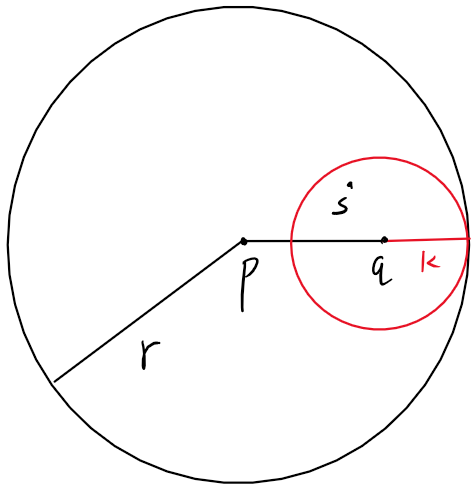
\includegraphics[scale=0.5]{linyushikaiji.png}
  \end{figure}

  \subsection{开集的补集}
  %相对开集与相对闭集
  $\forall E\subseteq X:$
  $$
  E^C\text{是闭集}\leftrightarrow E\text{是开集}
  $$
  \subsubsection{Démonstration}
  \subsubsection{Proposition}
  同理,补集是开集的集合是闭集.
  \subsection{Proposition: 开集的无限并与并集的无限交}
  $$
  \forall \alpha ,U_\alpha\text{是开集}\Rightarrow\bigcup_\alpha U_\alpha\text{是开集}
  $$
  $$
  \forall \beta ,E_\beta\text{是闭集}\Rightarrow\bigcap_\beta U_\beta\text{是闭集}
  $$
  \subsection{Proposition: 开集的有限交与并集的有限并}
  $$
  \forall \alpha ,U_\alpha\text{是开集}\Rightarrow\bigcup_\alpha U_\alpha\text{是开集}
  $$
  $$
  \forall \beta ,E_\beta\text{是闭集}\Rightarrow\bigcap_\beta U_\beta\text{是闭集}
  $$

  \subsection{闭包 L'adhérence}
  内点和极限点组成的几何叫做集合的闭包,记为$\overline{E}$即:
  $$
  \overline{E}=E\cup E'
  $$
  我们会给出一些关于闭包的简单的推论,它们都非常直观.
  \subsubsection{Exemple}
  $(114,514)$的闭包为$[114,514]$.
  \subsubsection{Remarque}
  闭包是闭集.
  \subsection{Proposition}
  与闭包相等的集合是闭集.
  $$
  E=\overline{E}\Leftrightarrow E\text{是闭集}
  $$
  \subsection{Proposition}
  集合$E$的闭包是包含它的最小闭集.
  \subsection{Proposition}
  对度量空间中的子集$E$,若:
  \begin{itemize}
    \item $E$有上界$\Rightarrow \sup E\in \overline{E}$
    \item $E$有下界$\Rightarrow \inf E\in \overline{E}$
  \end{itemize}
  \subsubsection{Démonstration}
  \noindent
  设$y=\sup E$.
  显然,若$y\in E$ 则$y\in \overline{E}$.\\
  若$y\notin E$ 则$\forall\epsilon>0\,\exists x\in E\, y-\epsilon<x<y $,也即$x\in N_\epsilon(y)\cap E$,则$y$是$E$极限点,故$y\in \overline{E}$.\
  $\inf$的证明一样.
  \subsubsection{Remarque}
  上述命题的逆命题不对.例如$[-114,0)\cup(0,514]$ 的上下界都属于该集合,但它不是闭集.
\section{相对开集/相对闭集}
  \subsubsection{Exemple}
  集合的开与闭受到其所在的度量空间的影响.设$E=(-3,3)$,则其在$\R$上是个开集,但是在$\R^2$上不是.
  这说明集合的开性质受到其所在度量空间的影响.为了消除这样的影响,我们需要讨论相对的开集和闭集.
  \subsection{相对开集}
  对度量空间$X$种的集合$E$和一点$q\in X$,若:
  $$
  \forall p\in E\,\exists r>0\,d(p,q)<r \Rightarrow q\in E
  $$
  则称$E$是$X$的相对开集.
  \subsection{Proposition}
  $Y\subseteq X\,,E\subseteq Y\,,G\in X$若$G$是开集,则:
  $$
  E=G\cap Y\Leftrightarrow E\text{是}Y\text{的相对开集}
  $$
  这个概念非常像\prettyref{myref:soustopo}提到的子空间拓扑.
  一个大空间里某个集合的性质仍属于这个集合和一个小空间交出来的集合.
  \subsection{相对闭集}
  对度量空间$X$种的集合$E$和一点$p\in X$,若:
  $$
  \forall p\in X\, \exists r>0\, N_r(p)\cap E\neq \varnothing\land N_r(p)\cap E\neq\{p\}\Rightarrow p\in E
  $$
  则称$E$是$X$的相对闭集.
  \section{紧集}%改到后面
    这部分内容放在这会显得很奇怪,因为在后面拓扑空间里我又会再讲一遍.
    但是为了Heine-Borel定理我又不得不讲清楚.
  \subsection{开覆盖}
  \subsubsection{有限子覆盖}
  \subsection{紧集}
  \subsection{相对紧致}
  \subsection{紧集的性质}
\section{Heine-Borel定理}
  \noindent
  OK,我们简单点,一上来我就把这个定理告诉你:\\
  对$E\subseteq \R^k\, k\in \mathbb{N}$,有:
  $$
  E\text{是紧集}\Leftrightarrow E\text{是闭集}\land E\text{是有界集}
  $$
  很显然,很直观,很一眼得出的结论.但是我们现在想要证明它可不简单.本节剩余的内容都是对这个重要定理的证明.
  \subsection{闭区间套性质}
  设$\R$中的一族闭区间$\{I_n \}\,, \forall n\in \mathbb{N}\,,I_n\subseteq I_{n+1}$,则有:
  $$
    \bigcap_{i=1}^\infty I_i\neq \varnothing
  $$
  闭区间套性质来源于$\R$的最小上界性.事实上这也是一种刻画实数集的方式,每个实数都是这样一族闭区间交集的极限.
  \subsubsection{Démonstration}
  证明非常简单,我已经给出了提示,就是最小上界性.设$I_i=[a_i,b_i]$,考虑闭区间下界组成的集合$E=\{a_i|i\in \mathbb{N}\}$,
  显然这个集合有上界(否则会得到$I_j=[a_j,b_j]\,b_j<a_j$),因此设最小上界$x=\sup E$.此外,$\forall i\in \mathbb{N}\,,b_i$也是$E$的上界,
  故有$x<b_i$,因此有$x\in[a_i.b_i]$.
  \subsection{$k$维格子}
  闭区间套性质不止是用于$\R$,而是可以类似地推广到$\R^k$.
  向量集
  $$\{\textbf{x}=(x_1,\dots,x_k)|x_j\in[a_j,b_j]_{j\in[\![1,k]\!]} \} $$
  称为$k$维格子.
  \subsubsection{Exemple}
  \begin{itemize}
    \item 1维格子就是上文提到的闭区间.
    \item 2维格子是一个封闭的矩形.
    \item 3维格子是一个长方体.
  \end{itemize}
  \subsection{$k$维格子的嵌套性质}
  设$\R^k$中的一族闭$k$维格子$\{I_n \}\,, \forall n\in \mathbb{N}\,,I_n\subseteq I_{n+1}$,则有:
  $$
    \bigcap_{i=1}^\infty I_i\neq \varnothing
  $$
  \subsubsection{Démonstration}
  这里的证明是闭区间套性质证明他推广,请读者自行尝试.只需要证明存在一组$x*=(x_1*,\dots,x_n*)$属于所有的$I_n$就行.

  \subsection{$k$维格子的紧致性}
  $k$维格子是紧集.
  \subsubsection{Démonstration}

  \subsection{Proposition}
  设$\R^k$中的子集$E$,则有:
  $$
  E\text{有界}\Leftrightarrow\exists I=\{\textbf{x}=(x_1,\dots,x_k)|x_j\in[a_j,b_j]_{j\in[\![1,k]\!]} \}\in \R^k\,, E\subseteq I
  $$
  \subsection{Heine-Borel定理}
  对$E\subseteq \R^k\, k\in \mathbb{N}$,有:
  $$
  E\text{是紧集}\Leftrightarrow E\text{是闭集}\land E\text{是有界集}
  $$
  \subsubsection{Démonstration}
  \noindent
  $\Rightarrow$:\\
  $\Leftarrow$:\\

  \subsection{实紧集的极限点}
  $\mathbb{R^k}$的子集$E$是紧集$\Leftrightarrow$$E$的每个无限子集在其中都有一个极限点.
  \subsubsection{Démonstration}
  \subsection{Weierstrass定理}

  \section{完备集与连通集}
  \subsection{Cantor三分集}
  \subsection{分离集}
  \section{压缩映射 Applications contractante}\label{myref:yasuoyingshe}

  

\chapter{赋范空间\\Espace Vectoriel Normé}
  这一章的核心概念是范数(模)的推广.把以前所学习的范数抽象化,然后推广应用.
\section{范数 La norme}
  范数是映射,也是泛函.对于以前学习过的模长,我们发现其具有非负性、绝对齐次性和三角不等式三个优秀的性质,于是我们将其提取出来并推广,重新定义范数.
  \subsection{Définition}
  给定映射:
  $$
  \Vert \cdot \Vert : \mathbb{E} \longrightarrow \R
  $$
  满足:\begin{itemize}
    \item 非负性:$\forall\alpha\in\mathbb{E}, \Vert \alpha \Vert\ge0$并且$\forall\alpha=0\Leftrightarrow \alpha=0_\mathbb{E}$.
    \item 绝对齐次性(homogénéité):$\forall\alpha\in\mathbb{E}, \Vert k\alpha \Vert=| k | \Vert \alpha \Vert$.这里$k$属于$\R$或者$\mathbb{C}$,具体由$\alpha$决定.
    \item 三角不等式(inégalité triangulaire):$\forall(\alpha,\beta)\in\mathbb{E}^2, \Vert \alpha+\beta \Vert\leq\Vert \alpha \Vert+\Vert \beta \Vert$.
  \end{itemize}
  即可称该映射是一个范数,并称$(\mathbb{E},N)$为一个赋范向量空间(sspace vectoriel normé)
  ,简称赋范空间,其中N为范数.
  \subsection{Remarque:线性}
  所谓齐次性,指的是$f(k\alpha)=kf(\alpha)$,绝对齐次性就是$f(k\alpha)= | k | f(\alpha)$.另外还有可加性$f(\alpha+\beta)=f(\alpha)+f(\beta)$.
  同时满足齐次性和可加性的运算称线性.为了明确乘法和加法,范数的公理化必须在线性空间内.
  \subsection{Proposition:范数诱导的度量}
  \subsection{平移不变性}


\section{$L^P$范数}\label{myref:LPnorme}
与讲义上的顺序不同,我打算直接定义$L^P$范数(又称为$P$范数)并研究它的性质,而不是通过需要的性质去定义三个范数.
  \subsection{Définition}
  对线性空间里的向量$\alpha=(a_1,a_2,\dots,a_n$),定义范数:
  $$
    \Vert \alpha\Vert_P=(\sum_{i=1}^{n}|a_i|^P)^{\frac{1}{P}},P\ge1  
  $$
  容易验证$L^P$范数的非负性和绝对齐次性,其三角不等式由Minkowski不等式得出.\\
  当$P=1$,$L^1$范数称曼哈顿(Manhattan)范数,诱导的度量称曼哈顿距离.这是因为曼哈顿的街道都建得方方正正,从街道上一点到另一点的距离基本上就是走出两条垂直的线的长度.\\
  当$P=2$,$L^2$范数称即是通常意义下的范数,诱导的也就是通常意义下的距离\\
  当$P\rightarrow \infty$,$L^\infty$范数称一致范数(或者上确界范数),诱导的度量称切比雪夫(Chebyshev)距离,又叫棋盘距离.两点之间的距离是其各个坐标数值中绝对值最大的那一个.
  显然,这是因为$\Vert \alpha\Vert_\infty=\max\{|a_i|\}$\\
  当$P<1$时,Minkowski不等式不成立,需要反号,无法定义范数,但仍然有许多有趣的性质.
  \subsection{开球 La boule ouverte}
  \subsubsection{Définition}
  赋范空间$(E,\Vert \cdot \Vert)$中,有$q\in E,r\in(0,+\infty)$,对于集合:
  $$
    B(q,r)=\{x\in E |\Vert x-q \Vert<r \}
  $$
  称$B$是以$q$为中兴半径$r$的开球.请对照\prettyref{myref:voisinage},开球与邻域的区别,其实就是度量和范数的差异.
  \subsection{单位球与等距线}
  称$B(0,1)$为赋范空间$(E,\Vert \cdot \Vert)$上的单位球(boule unité).作距离为1的各范数的等距线:
  \begin{figure}[H]%插入题目的图片
    \centering
    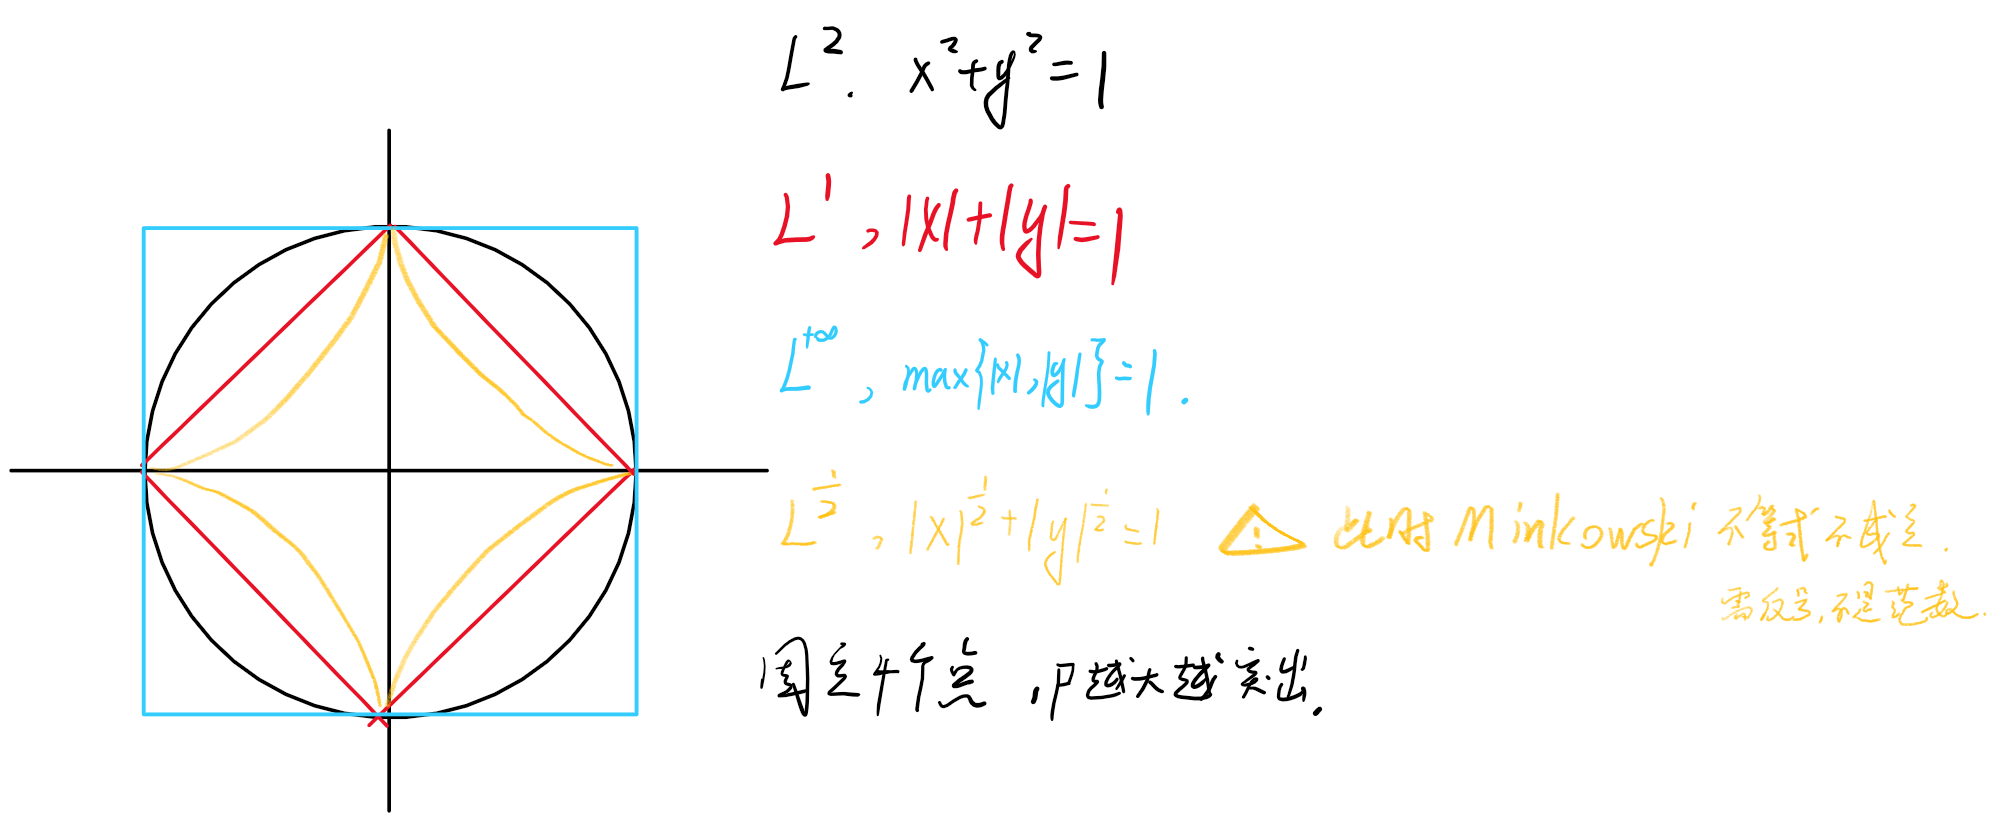
\includegraphics[scale=0.6]{danweiqiu.png}
    \label{fig:1}
  \end{figure}
  特别说明,我这里给出了$P=\frac{1}{2}$的情况,用来说明,对于单位球,其实就是固定4个点,然后P越大曲线越往外凸.
  \subsection{函数空间上的$L^P$范数}
  既然有了Euclide空间上的$L^P$范数,我们自然也会想在其他空间上玩玩这个.最熟悉的空间莫过于函数空间了!
  仿照之前的$L^P$范数,我们发现,不太好给函数又加和又开方什么的.但是所幸我们有一个替代方案,那就是同样非常熟悉的Riemann积分!
  \subsubsection{Définition}
  对$\C ^0I$上的函数$f$,定义范数:
  $$
  \Vert f \Vert_P=(\int_{I}|f(x)|^P \mathrm{d} x)^{\frac{1}{P}},P\ge1
  $$
  这样就得到了函数空间上的$L^P$范数!
  \subsubsection{Remarque}
  我们发现,当$P\rightarrow \infty$时$L^\infty$范数$\Vert f \Vert_\infty=\max|f(x)|,x\in I$,这正是函数$f$在$I$上的上确界.
  现在回顾之前我们对一致收敛的定义,那里提到的$\Vert f_n-f \Vert_\infty\rightarrow 0$就非常好理解了.
\section{空间的完备化}
  (Introduction)让我们先通过一个例子引出完备空间.
  \subsection{实数:七个等价命题}
  我们说"实数$\R$是完备的",这对应于七个等价的命题.这些命题可以相互推导:
  \begin{itemize}
    \item Dedekind分割定理
    \item 确界原理
    \item Heine-Borel定理
    \item 单调收敛定理
    \item 闭区间套定理
    \item Bolzano-Weierstrass定理
    \item Cauchy收敛原理
  \end{itemize}
  这其中,AAAAA是本讲义已经介绍过的内容,剩余的(带介绍).

  在这七个命题里,Cauchy收敛原理应为只涉及了度量,故比较容易用来达成我们的完备化步骤.我们将通过这一原理来详细阐述一个度量空间的完备化
  \subsection{收敛}
  当我们尝试把范数、度量、内积等等概念都抽象化、公理化地定义了之后,是时候重新回顾一下,一个重要概念——收敛了.
  当然,课程的内容只在赋范空间内讨论了收敛,所以我们先看赋范空间内的.
  我们会尝试用精确的$\epsilon-\delta$语言来定义它:
  \subsubsection{Définition}
  赋范空间$(E,\Vert \cdot \Vert)$中,点列$(u_n)_{n\in\mathbb{N}},l\in E$,若:
  $$
    \forall\epsilon>0, \exists p\in \mathbb{N}, n\ge p\Rightarrow \Vert u_n-l \Vert<\epsilon
  $$
  称$(u_n)_{n\in\mathbb{N}}$在$(E,\Vert \cdot \Vert)$中收敛于$l$.
  \subsection{Proposition}
  若$(u_n)_{n\in\mathbb{N}}$在$(E,\Vert \cdot \Vert)$中收敛于$l$,则$(u_n-l)_{n\in\mathbb{N}}$在$(E,\Vert \cdot \Vert)$中收敛于$0$.
  \subsection{Proposition}
  若$(u_n)_{n\in\mathbb{N}}$在$(E,\Vert \cdot \Vert)$中收敛于$l_1$和$l_2$,且二者同属于赋范空间$(E,\Vert \cdot \Vert)$,则$l_1=l_2$
  
  
  \subsection{Cauchy列与收敛}
  下面我们进入到度量空间,利用Cauchy列讨论完备.
  \subsubsection{Définition}
  度量空间$(X,d)$中,点列$(u_n)_{n\in\mathbb{N}}$,若:
  $$
    \forall\epsilon>0, \exists p\in \mathbb{N}, m>p,n>p\Rightarrow d(u_m,u_n)<\epsilon
  $$
  称点列$(u_n)_{n\in\mathbb{N}}$是一个Cauchy列.
  \subsubsection{Proposition}
  度量空间中收敛的点列一定是Cauchy列.
  \subsubsection{Proposition}
  度量空间中的Cauchy列一定有界.
  \subsubsection{Proposition}
  子列收敛的Cauchy列一定收敛.


  \subsection{再论闭包与稠密集}
  \subsubsection{闭包}
  现在我们可以尝试把集合拖到赋范空间里,尝试定义集合的闭包.
  对赋范空间$(E,\Vert \cdot \Vert)$中的集合$A$,定义其闭包为:
  $$
    \overline{A}=\{x\in E | \forall(a_n)\in A^\mathbb{N},a_n\xrightarrow[n\rightarrow+\infty]{}x\}
  $$

  \subsubsection{Proposition}
  赋范空间$(E,\Vert \cdot \Vert)$中的集合$A\in\overline{A}$.
  \subsubsection{稠密集}
  对赋范空间$(E,\Vert \cdot \Vert)$和其中的集合$A$,如果:
  $$
    \forall x\in E, \exists (a_n)\in A^\mathbb{N}, a_n\xrightarrow[n\rightarrow+\infty]{}x
  $$
  称集合$A$在$E$上是稠密的.显然,常见的如有理数集在实数集上仍然是稠密的.
  \subsubsection{Bonus}
  Pierre曾在某次作业里要求证明无理数集在$\R$上稠密.当你学了这里的定义之后应该就非常简单了.当时我是这么写的:\\

    Soit $\mathbb{I} =\R\setminus \mathbb{Q}$.
    $\forall x\in \R$:\\
    \indent
    Si $x\in \mathbb{I}$, 
    soit une suit $\left \{ \alpha_n \right \}=x \Rightarrow 
    \lim_{n \to \infty}x=x\in \mathbb{\overline{I}}$.\\
    \indent
    Si $x\in \mathbb{Q}$, 
    soit une suit $\left \{ \beta_n \right \}=x-\frac{\sqrt{2}}{n}$. 
    $\forall n\in \mathbb{N}, \beta_n=x-\frac{\sqrt{2}}{n}\in \mathbb{I}$ et 
    $\lim_{n \to \infty}\beta_n=x\in \mathbb{\overline{I}}$.\\
    \indent
    Donc $\forall x\in \R, \exists (a_n)_{n\in\mathbb{N}}\in \mathbb{I}^{\mathbb{N}}, n\xrightarrow[a_n\rightarrow\infty]{}x$. 
    Cela dit que $\mathbb{I}=\R\setminus \mathbb{Q}$ est dense dans $\R$.\\


  \subsection{完备空间与完备化 }
  \subsubsection{Définition}
  若度量空间$(X,d)$中任意一个Cauchy列都收敛,称度量空间$(X,d)$是完备的(complet)度量空间.
  称完备的赋范空间为Banach空间,完备的内积空间为Hilbert空间.想要熟悉这两个空间的具体性质就去学习泛函分析吧.\\

  把一个度量空间加上其Cauchy列的极限点组成的最小度量空间这一过程称为对度量空间的完备化.例如,有理数集的完备化就是实数集.

\section{等价度量与等价范数 }  \label{myref:normeq}
  \subsection{双Lipschitz条件 }
  给定两个度量空间$(E_1,d_1),(E_2,d_2)$,集合$U\subseteq E_1$.
  若对于函数$f:U\rightarrow E_2$存在常数$K$使得对任意集合$U$中的元素$(a,b)$有:
  $$
  d_2(f(a),f(b))\leq Kd_1(a,b)
  $$
  称该函数符合Lipschitz条件.\\
  若存在$K\ge 1$使得:
  $$
  \frac{1}{K}d_1(a,b)\leq d_2(f(a),f(b))\leq Kd_1(a,b)
  $$
  称该函数符合双Lipschitz条件.
  \subsection{等价范数 La norme équivalente}
  \subsubsection{Définition}
  设线性空间$E$上的两个范数$N_1$和$N_2$若:
  $$
    \exists(a,b)\in(0,+\infty),\forall x\in E,aN_1(x)\leq N_2(x)\leq bN_1(x)
  $$称$N_1$和$N_2$是等价(équivalente)范数.
  \subsubsection{Remarque}
  等价范数是等价关系,具有自反性、传递性和对称性.
  \subsubsection{Proposition}
  n维线性空间上的所有范数等价.

\chapter{内积 Produit Scalaire}
  这一部分是在小学期讲的.
    \subsection{Définition}
    \subsection{Cauchy-Schwatz不等式}
    \subsection{内积诱导的范数}
    \subsection{平行四边形等式}


\chapter{拓扑空间\\ Espace Topologique}
拓扑是什么?拓扑学内容有哪些?拓扑这个词或许经常听到,但是对于具体的含义和内容想必不是很了解.
事实上,从度量开始,就已经可以算是拓扑学的内容了,我们已经学习了好几章的拓扑学,只不过到了这一章才正式地把这些概念定义出来.
之前我们完成了距离的公理化、模长的公理化和内积的公理化,拓扑也是一个我们熟悉的概念公理化,那就是开集.
拓扑研究的就是开集的集族(Famille d'ensembles).
\section{拓扑空间}
  与度量空间、赋范空间和内积空间类似,拓扑也有对应的拓扑空间,定义如下:
  \subsection{Définition}
  给定集合$X$和集族$\tau $,满足:
  $$
  \begin{aligned}&
  1.\varnothing\in\tau , X\in\tau\text{,空集和全集是开集}\\&
  2.\forall\alpha\in I,U_\alpha\in\tau \Rightarrow\bigcup_{\alpha\in I}U_\alpha\in\tau \text{,开集的并集是开集.}\\&
  3.\forall n\in\mathbb{N},\bigcap_{i=1}^{n}U_i\in\tau \text{,开集的有限交是开集.}\\
    \end{aligned}
  $$
  则称$\tau $是$X$上的一个拓扑,称$(X,\tau)$是一个拓扑空间,$U$称其中的开集.
  \subsection{Remarque:其他的公理化}
  除了以上的公理化方式,还有两种常见的拓扑定义.
  \subsection{Proposition:闭集}
  由de Morgan定律得:
  $$
  \begin{aligned}&
  1.\varnothing, X{ 是闭集.}\\&
  2.\forall\alpha\in I,E_\alpha\text{是闭集} \Rightarrow\bigcap_{\alpha\in I}E_\alpha \text{是闭集.闭集的交是闭集.}\\&
  3.\forall n\in\mathbb{N},\bigcup_{i=1}^{n}E_i \text{是闭集.闭集的有限并是闭集.}\\
    \end{aligned}
  $$
  \subsection{Exemple}
  $\R$上的所有形如$[a,b)$的区间可以组成一个拓扑,其中每个$[a_i,b_i)$都是开集.

  \subsection{离散拓扑 Topologie discrète}
  离散拓扑即$\tau=\mathcal{P} (X)$,其拓扑是集合的幂集,也就是其所有子集的集族.
  离散拓扑空间里所有的单点集都既是开集又是闭集,相互之间都是"孤立的".

  \subsection{密着拓扑 Topologie grossiète}
  密着拓扑即$\tau=\{X,\varnothing \}$,又叫不可分拓扑,其空间里只有空集和整个空间是开集,所有的点都被"粘在一起",无法通过拓扑的方式区分开来.\\
  
  可以认为,离散拓扑和密着拓扑是两个"极端的"拓扑,全包和全不包.
  也正因为其极端性,它们有着一些特殊的性质,我们在后续研究.
  
  \subsection{度量诱导的拓扑}
  对$(X,\tau)$,若存在度量$d$可以定义拓扑的开集,称$(X,\tau)$是可度量的(英:metrizable).
  例如,\prettyref{myref:lisanduliang}的离散度量可以诱导离散拓扑,此时邻域$N_\frac{1}{2}=\{X\}$就是开集.
  而对于card$(X)>1$的密着拓扑就无法被度量.
  \subsection{有限补拓扑 Topologie des compléments finis}
  有限补拓扑中,补集有限的集合是开集.即$\tau=\{U|U\subseteq X,U^C\text{是有限集} \}\cup \{\varnothing\}$

  \subsection{子空间拓扑}\label{myref:soustopo}
  提前预告一下,这是个简单但是非常重要的概念,我们在后面的证明中会多次用到这个概念.\\
  对$(X,\tau)$,$Y$是$X$的子集,则存在一个拓扑$\tau_y=\{Y\cap U| U\in\tau\}$,也就是说,拓扑与子集的交集可以组成一个新的拓扑.
  \subsubsection{Démonstration}
  $$
  \begin{aligned}&
  \varnothing\cap Y=\varnothing\in\tau_y\\&
  X\cap Y=Y\in\tau_y\\&
  \bigcup_{\alpha\in I}(U_\alpha\cap Y)=(\bigcup_{\alpha\in I}U_\alpha)\cap Y\in Y\\&
  \bigcap^n_{i=1}(U_i\cap Y)=( \bigcap^n_{i=1}U_i)\cap Y\in Y
  \end{aligned}
  $$
  \subsubsection{Exemple}
  对于$\R$上的常规拓扑和子集$Y=[0,+\infty),\forall (a,b)\in\R,(a,b)\cap[0,\infty)\in\tau_y$.
\section{拓扑空间里的点集}
  现在让我们来看一看那些以前很熟悉的概念拿到拓扑空间里之后会发生什么.
  \subsection{邻域}
  对$(X,\tau)$中的一点$x$,若存在开集$U\in\tau, x\in U$,则称$U$是$x$的一个邻域,记为$U(x)$,$U/x$是$x$的去心邻域,记为$\check{U}(x) $.
  注意到,现在的邻域跟之前的在对称性上有所差异,之前我们规定一个点的邻域好像都是关于这个点"对称"的,点在邻域的正中央,现在这个点可以在邻域里的任意位置.
  我当初学到这里也觉得奇怪,但是后面一想,也没用上这个所谓的对称性啊,所以其实问题不大.
  \subsection{内点}
  $(X,\tau), E\subseteq X,x\in E,\text{若存在} U(x)\subseteq E$则称呼$x$是$E$的一个内点. $E$的所有内点组成的集合称为其内部,记为$E^O$.
  \subsection{极限点与闭包点}
  $(X,\tau), E\subseteq X,x\in E$若有$\forall\check{U}(x)\cap E\neq\varnothing$,则$x$是$E$的极限点.$E$的所有极限点组成的集合称为导集,记为$E'$.同理,
  若有$\forall U(x)\cap E\neq\varnothing$,则$x$是$E$的闭包点.$E$的所有闭包点组成的集合称为闭包,记为$\bar{E}$.
  熟悉的感觉又回来了.同样,我们可以证明$\bar{E}=E\cup E'$.
  \subsection{外点与边界点}
  与内点这个概念相对应,考虑$E$的补集$E^C$,将其内点称为$E$的外点,组成的集合称为外部,记为$E^e$.不是内点又不是外点的点称为边界点,组成的集合称为边界,记为$\partial E$.
  \subsection{熟悉的命题}
  把以前的一些命题拿过来放到拓扑空间,它们仍然成立.
  \begin{itemize}
    \item $U\text{是开集}\Leftrightarrow U=U^O$,内部等于自身的集合是开集.
    \item $U^O=(U^O)^O$,内部是开集.
    \item $U^O$是包含于$U$的最大开集.
    \item $E\text{是闭集}\Leftrightarrow E=\bar{E}$,闭包等于自身的集合是闭集.
    \item $\bar{E}=\bar{\bar{E}}$,闭包是闭集.
    \item $\bar{E}$是包含于$E$的最小闭集.
  \end{itemize}
  \subsubsection{Démonstration}
  待补充,笔记上的太乱了.




\section{拓扑空间里的收敛 }
  现在我们要在拓扑空间中再次研究这个重要的,贯穿了大量分析学内容的概念————收敛.
  \subsection{Définition}
  $(X,\tau)$中的点列$\{a_n\}$和一点$x$,若有:
  $$
  \forall U(x), \exists N\in \mathbb{N}*\text{使得}n>N\Rightarrow a_n\in U(x)
  $$
  称点列$\{a_n\}$收敛于点$x$.
  \subsubsection{Exemple}
  $X=\{a,b,c\},\tau =\{\varnothing, X, \{a,b\}, \{a,c\}, \{a\}\},a_n\equiv a$.则有$\{a_n\}$收敛于点$a$.
  \subsubsection{Remarque:收敛不唯一}
  注意到,在上述的条件里,点列的收敛是不唯一的!!!因为$\{a,b\}$也是点$a$的邻域,所以$\{a_n\}$收敛于点$b$;$\{a,c\}$也是点$a$的邻域,所以$\{a_n\}$收敛于点$c$.也就是说,$\{a_n\}$同时收敛于$a,b,c$三个不同的点!
  这多么可怕,与我们之前见过的只收敛到一个点的收敛概念完全不同.出现这一情况,是因为在之前我们学习的空间里,两个点之间存在没有交集的邻域,但是在拓扑空间里这条法则失效了,所以收敛有了这样的奇怪的性质.
  然而这不是什么好的性质,如果点列的收敛是不唯一的,那我们就无法区分收敛到的哪些点了,点集拓扑的探讨也就失去了意义.
  所以这一个收敛的定义其实不重要,因为没什么用.我们必须对它加以改进,添加更多的限制条件来确保能有效运用收敛.
  \subsection{Hausdorff条件:$T_2$公理}
  对$(X,\tau)$中任意两点$x_1,x_2$,若:
  $$
    \forall(x_1,x_2)\in X^2, x_1\neq x_2, \exists U(x_1),U(x_2)\text{使得}U(x_1)\cap U(x_2)=\varnothing
  $$
  则称$X$是一个Hausdorff空间.该条件又称为拓扑空间里的分离公理,或者$T_2$公理,它把空间里的点分离开了.
  \subsubsection{Proposition}
  一个有限集是一个Hausdorff空间,当且仅当它的$\tau$是离散拓扑.
  \subsubsection{Démonstration}
  离散拓扑的有限集显然是Hausdorff空间.我们证明另一个方向,利用反证法:
  $$
  \begin{aligned}&
    \lnot (\tau\text{是离散拓扑})\Rightarrow \exists x\in X, \{x\}\notin \tau\\&
    \text{设}x \text{的所有邻域交集为}\mathbb{U}\Rightarrow\mathbb{U}\cap x\neq\varnothing \\&
    \text{设}y\in\mathbb{U}\cap x\\&
    \Rightarrow \forall U(y)\cap\mathbb{U}\neq\varnothing\\&
    \Rightarrow \forall U(y),\forall U(x),U(y)\cap U(x)\neq\varnothing\\&
    \Rightarrow X\text{不是Hausdorff空间}
    \end{aligned}
  $$
  所以我们发现,如果研究有限集,那就绕不开离散拓扑,研究其收敛性也就没什么意义了.
  \subsubsection{Proposition}
  Hausdorff空间里点列的收敛具有唯一性,即$\{a_n\}$收敛于点$x$和$y\Rightarrow x=y$.
  \subsection{Hausdorff空间里的闭集}
  Hausdorff空间里单点集都是闭集.
  \subsubsection{Démonstration}
  对于Hausdorff空间里一点$x$,有:
  $$
  \forall y\in x^C, \exists U(y)\cap x\neq\varnothing\Rightarrow U(u)\subseteq x^C\Rightarrow y\in(x^C)^O
  $$因此$x^C$是个开集,那$x$自然就是个闭集了.
  \subsubsection{Proposition}
  Hausdorff空间里有限集都是闭集.
  \subsubsection{Proposition}
  度量空间都是Hausdorff空间.

  \subsection{Fréchet条件:$T_1$公理}
  在证明Hausdorff空间里单点集都是闭集的时候,我们用到了这样一步:
  $$
  \exists U(y)\cap x\neq\varnothing
  $$
  对比Hausdorff条件本身,我们发现这里没有用全.我们只用了点和邻域的关系而不是邻域和邻域的关系,这说明Hausdorff条件是一个很强的条件,我们可以尝试再稍微弱化一下它.
  于是就有了Fréchet条件:单点集都是闭集的拓扑空间称为Fréchet空间.





  \subsection{$T_0$公理与Kolmogorov体系}
  这里重新调整一下

  \section{拓扑公理体系 Systeme d'axiomes topologiques}
  \subsection{$T_0$ Kolmogorov 公理 Axiome de Kolmogorov}
  \subsection{$T_1$ 公理 Axiome de Fréchet}
  \subsection{$T_2$ Hausdorff 公理 Axiome de Hausdorff}
  \subsection{$T_3$ 正规公理 Axiome régulier}
  \subsection{$T_4$ 公理 Axiome complètement régulier}
  \subsection{$T_5$ 公理 Axiome complètement régulier de Hausdorff}
  \subsection{$T_6$ 公理 Axiome dénombrable}
  \subsection{$T_7$ 公理 Premier axiome dénombrable}
  \subsection{$T_8$ 公理 Deuxième axiome dénombrable}
  \subsection{$T_9$ 公理 Axiome de Lindelöf}


\section{连续性与映射}
  现在,我们继续公理化拓扑空间里映射的连续性.
  \subsection{Définition}
  考虑两个拓扑空间$(X,\tau_x)(Y,\tau_y)$上的映射$f:X\rightarrow Y$,若:
  $$
  \forall U\in\tau_y,f_{-1}(U)\in\tau_x
  $$
  则称映射$f$是连续的.
  \subsection{拓扑的选择与连续性}
  对于同一个集合,我们选择不同的拓扑,则可能导致连续性的改变.
  例如,设$\R_d$是$\R$上的离散拓扑,$\R_n$是$\R$上的通常拓扑,$f(x)=x$是恒等映射,则:
  \begin{itemize}
    \item $f:\R_n\rightarrow \R_d$不是连续映射,单点集在$\R_n$上不是开集.
    \item $f:\R_d\rightarrow \R_n$是连续映射.
  \end{itemize}
  \subsection{由公理推导而来的等价命题}
  一下命题等价,它们分别对应着不同的拓扑公理.这也说明拓扑公理是可以相互转化的.
  \begin{itemize}
    \item 1.$\forall U\in\tau_y,f_{-1}(U)\in\tau_x$.(开集公理)
    \item 2.$\forall E\subseteq X,f(\bar{E})\subseteq \bar{f(E)}$.(闭包公理)
    \item 3.$\forall E\in Y\text{是闭集},f_{-1}(E)\in X\text{是闭集}$.(闭集公理)
    \item 4.$\forall x\in X, \forall U[f(x)], \exists U(x)\text{使得}f[U(x)]\subseteq U[f(x)]$.(邻域公理)
  \end{itemize}
  \subsubsection{Démonstration}
  $1\Rightarrow 2$:
  $$
  \begin{aligned}&
    \forall x\in \bar{E},f^{-1}U[f(X)]\cap E\neq\varnothing\\&
    \Rightarrow U[f(x)]\cap f(E)\neq\varnothing\Rightarrow f(x)\in \bar{f(E)}
    \end{aligned}
  $$


  $2\Rightarrow 3$:
  $$
  \begin{aligned}&
    \forall x\in \bar{f^{-1}(E)},f(x)\in \bar{E}\\&
    \Rightarrow x\in f^{-1}(E)\Rightarrow\bar{f^{-1}(E)}\subseteq f^{-1}(E)\\&
    \Rightarrow f^{-1}(E)\text{是闭集}
    \end{aligned}
  $$


  $3\Rightarrow 1$:
  $$
  \begin{aligned}&
    U\subseteq \tau_y\Rightarrow U^C\text{是闭集}\Rightarrow f^{-1}(U^C)\text{是闭集}\\&
    \Rightarrow f^{-1}(U^C)=[f^{-1}(U)]^C\Rightarrow f^{-1}(U)\in\tau_x
    \end{aligned}
  $$


  $4\Rightarrow 1$:
  这里的证明其实就是前面证明过的东西反过来,留给读者完成.
  \subsection{Exemple}
  接下来给出几个连续映射
  \subsubsection{常值映射 }
  $$
    f:X\rightarrow  Y
  $$
  $$
    x\rightarrow C
  $$
  $\forall \text{开集}U\subseteq Y,C\in U\Rightarrow f^{-1}(U)=X \text{是开集}, 
  C\notin U\Rightarrow f^{-1}(U)=\varnothing \text{是开集}$,故常值映射是连续映射.
  \subsubsection{包含映射 }
  包含映射是$X$的子集$A$上的恒等映射
  $$
    i:A\hookrightarrow  X
  $$
  $$
    x\rightarrow x
  $$
  $\forall \text{开集}U\subseteq X,i^{-1}(U)=U\cap A \text{是开集(子空间拓扑)}$,故常值映射是连续映射.
  \subsubsection{复合映射 }
  给定连续映射$f:X\rightarrow  Y\text{    }g:Y\rightarrow  Z$,其复合映射
  $$
    \phi:X\rightarrow Z
  $$
  $$
    x\rightarrow g(f(x))
  $$
  也是连续映射.$\forall \text{开集}U\subseteq Z,g^{-1}(U)\subseteq Y 
  \text{是开集}\Rightarrow f^{-1}(g^{-1}(U))\subseteq X\text{是开集}\Rightarrow (f\circ g)^{-1}(U)\text{是开集}$,
  故连续映射的复合映射也是连续映射.
  \subsubsection{限制映射 }
  考虑连续映射$f:X\rightarrow Y$,对$A\subseteq X:$
  $$
  f|_A:A\rightarrow Y
  $$
  $$
    x\rightarrow f(x)
  $$
  为连续映射(考虑包含映射和映射$f$的复合映射即可).
  \subsubsection{陪域缩小}
  考虑连续映射$f:X\rightarrow Y$,对$Z\subseteq X:$
  $$
    f': X\rightarrow Z
  $$
  $$
    x\rightarrow f(x)
  $$
  则$f'$也是连续映射(考虑映射$f$和包含映射的逆映射的复合映射即可).
  \subsubsection{陪域扩大}
  考虑连续映射$f:X\rightarrow Y$,对$Y\subseteq Z:$
  $$
    f': X\rightarrow Z
  $$
  $$
    x\rightarrow f(x)
  $$
  则$f'$也是连续映射(考虑映射$f$和包含映射的复合映射即可).
  \subsection{局部表示与粘接原理 }
  在讨论拓扑空间上的连续函数时,我们不必要求直观地看出整个函数都是连续的,而是可以间接地"拼凑"出一个连续函数.
  若我们采用开集"拼凑",则这个过程称为连续性的局部表示;若采用闭集,则称为粘接原理.即对拓扑空间上的函数$f:X\rightarrow Y$:
  $$
    X=\bigcup_{\alpha\in I}U_\alpha ,\forall \alpha\in I, U_\aleph\text{是开集}
  $$
  $$
  \forall \alpha\in I,f|_{U_\alpha}:U_\alpha\rightarrow Y\continue\Rightarrow f:X\rightarrow Y\continue
  $$
  即为连续性的局部表示;
  $$
    X=\bigcap_{i=0}^{n}V_i ,\forall i\in[\![0,n]\!], V_i\text{是闭集}
  $$
  $$
    \forall i\in[\![0,n]\!],f|_{V_i}:V_i\rightarrow Y\continue\Rightarrow f:X\rightarrow Y\continue
  $$
  \subsubsection{Démonstration}
  \begin{figure}[H]%插入题目的图片
    \centering
    
\includegraphics[scale=0.2]{proofforreader.jpg}
  \end{figure}


\section{同胚 Homeomorphisme}\label{myref:tongpei}
  现在我们来到了拓扑里面最重要的概念——同胚.你可能听过这个著名的笑话:\\

  一个拓扑学家把咖啡倒进了甜甜圈里.有人问他为什么不把咖啡倒进咖啡杯里,拓扑学家非常惊讶:"它们有什么区别?不是同胚的吗?"
  \subsection{Définition}
  对拓扑空间上的映射$f:X\rightarrow Y$若$f$满足:
  \begin{itemize}
    \item $f$是双射
    \item $f$是连续映射
    \item $f^{-1}$是连续映射
  \end{itemize}
  则称$f$是$X$到$Y$上的一个同胚映射,此时$X$和$Y$是同胚的.显然,同胚是一个等价关系.
  \subsection{Exemple}
  \subsection{Remarque}
  请回顾我们在\prettyref{myref:Homomorphisme}和\prettyref{myref:Isomorphisme}里提到的同态和同构,它们有什么相似的地方?\\

  在拓扑空间上前两条无法推出第三条性质,我们讲马上给出一个经典的反例用来说明这一点.
  \subsection{Exemple: 反例}
  给出由半开半闭区间$[0,1)$到单位圆上的映射
  $$
  f:[0,1)\rightarrow \{(x,y)|x^2+y^2=1\}
  $$
  $$
  x\mapsto\cos(2\pi x)+\sin(2\pi x)
  $$
  $f$是连续的双射,但是$f^{-1}$在$(1,0)$处不连续.
  这是因为我们把区间的两端"粘贴"了起来,这导致了拓扑性质的改变,因此无法保持同胚.事实上,只要进行了类似"粘贴""裁剪"或者"穿孔"等等操作,原来的拓扑就变了.
  这些操作会在拓扑学里严格定义,这里不再谈论.
  \subsection{Proposition}
  对$\R$上的一元函数$f:X\rightarrow Y$,有:$X,Y$是$\R$上的两个区间(不能是子集!).若:
  \begin{itemize}
    \item $f$是双射
    \item $f$是连续映射
  \end{itemize}
  则$X,Y$同胚.
  \subsection{Exemple: 反例}
  若上述推论里将\textbf{$X,Y$是$\R$上的两个区间} 改成 \textbf{$X,Y$是$\R$上的两个子集} ,则结论不成立.
  例如映射$f:X\rightarrow Y$有 $X=[0,1]\cup(2,3],Y-[0,2]$
  $$
  x\mapsto 
  \begin{cases}
    x &x\in[0,1]\\
    x-1 &x\in (2,3]
    \end{cases}
  $$
  则$f^{-1}$不连续.
  \subsection{Proposition}
  对双射$f:X\rightarrow Y$,若:
  $$
  U\text{是$X$上的开集}\Leftrightarrow f(U)\text{是$Y$上的开集}
  $$
  则$X,Y$同胚.

  \section{紧致性与列紧性 Compacité et séquentialité}
  \subsection{拓扑不变量 Topological invariant}
  与同构类似,同胚的拓扑空间也有一些不会变化或者相等的东西.这些东西被称为拓扑性质或者拓扑不变量.
  它们在同胚映射下保持不变.由于许多概念还没有讲到,我们仅仅给出拓扑不变量的概念,以便于大家理解拓扑空间上的紧致性.
  更多的拓扑不变量将在拓扑学中研究.
  \subsection{Remarque}
  我们将以前所学过的度量空间上的开覆盖推广到拓扑空间.这并没有难度,因为拓扑空间直接就是拿开集定义的,不需要额外添加什么内容.
  对拓扑空间$X$上的开集族$\{U_\alpha|\alpha\in I \}$满足
  $$
    X\subseteq \bigcup_{\alpha\in I}U_\alpha
  $$则称$\{U_\alpha\}$是拓扑空间$X$上的一个开覆盖.\\

  同理,若能找到一组有限个开集覆盖$X$,即A和B拥有相同的基数
  $$
  X\subseteq \bigcup_{i=1}^{n}U_i
  $$则称$\{U_\alpha\}$是拓扑空间$X$上的一个有限开覆盖/有限子覆盖.
  \subsection{Définition: 紧致}
  对拓扑空间$X$上的任意一个开覆盖,若都能找到一个有限子覆盖,则称$X$是一个紧致空间,或称$X$是紧的.
  若$Y\subseteq X$也是紧的,则称$Y$是一个紧致集/紧集.
  \subsection{Définition: 序列紧致}
  对拓扑空间$X$上的任意一个序列,若都能找到一个子序列$\{ x_n\}$收敛于$x\in X$,则称$X$是一个序列紧致空间,或称$X$是列紧的.
  若$Y\subseteq X$也是列紧的,则称$Y$是一个列紧集.
  \subsection{Remarque}
  或许你还记得我们在度量空间上讨论的紧致性问题,当时我们并没有这么区分紧和列紧.
  事实上,在度量空间上,紧致性和列紧性是等价的,这两个概念都起源于Bolzano对于收敛子列的研究.
  在研究收敛性上,发展出了Bolzano-Weierstrass定理和Arzela-Ascoli定理等对于序列紧致性的结论;
  在研究连续性上,又发展出了Heine-Borel定理作为连续性的结论.
  早期的列紧性比紧致性更为直观(显然,度量下的点列收敛肯定比开集更加容易直观理解),因此Fréchet将现在的列紧性定义为紧致.
  但是后来随着拓扑空间研究的深入,人们发现两者不等价,且在拓扑空间上Heine-Borel利用开区间表示的紧致性更容易理解,更何况在一般的拓扑空间下无法讨论序列的收敛,
  因此最终由Pavel和Urysohn用Heine-Borel的方法定义紧致性,而将Bolzano-Weierstrass的方法定义为列紧性.在本章中,我们主要考虑紧致性的问题.
  \subsection{Proposition}
  $Y$是$X$上的一个紧致集等价于以下表述:
  $$
  \text{对开集族 }\{U_\alpha\}\subseteq X, \{U_\alpha\}\text{是 }Y\text{的开覆盖 }\Rightarrow
  \exists\{U_i|i\in[\![1,n]\!]\}\subseteq\{U_\alpha\}\text{是 }Y\text{的有限子覆盖 }
  $$
  这说明了一个很重要的结论:集合的紧致性与其在什么空间上无关.一个紧的$Y$放在任何$X$里都是紧的.
  \subsection{Exemple}
  \subsubsection{1.  $\R$既不紧,也不列紧}
  我们可以找到开覆盖
  $$
  C=\{(n,n+2)|n\in\mathbb{Z}\}
  $$
  从中拿去任意一个区间之后就无法覆盖$\R$了.\\
  对于$\R$趋近于正无穷的子列显然不收敛于$\R$上的某个点.
  \subsubsection{2.  $(0,1]$既不紧,也不列紧}
  \subsubsection{3.  $\{0\}\cup \{\frac{1}{n}|n\in\mathbb{N}\}$既紧,也列紧}
  \begin{figure}[H]%插入题目的图片
    \centering
    
\includegraphics[scale=0.2]{proofforreader.jpg}
  \end{figure}
  \subsection{紧集的投影}
  定义投影算子$\mathcal{P}:X^2\rightarrow X$
  $$
  (a,b)\mapsto a
  $$
  若$A^2$紧致,则$\mathcal{P}(A)$也紧致.
  \subsection{Proposition}
  两个紧集的笛卡尔积同样是紧集.
  $$
  A\times B\text{是紧集}\Leftrightarrow A\text{是紧集}\land B\text{是紧集}
  $$
  \subsection{Proposition}
  有限个紧集的笛卡尔积同样是紧集.(此时不能反推)
  $$
  A_1,\dots,A_n\text{是紧集}\Rightarrow A_1\times \dots\times A_n\text{是紧集}
  $$
  \section{闭集刻画的紧致集}
  利用闭集刻画紧致集,可以在一定程度上简化我们的计算和证明.
  \subsection{Remarque: 有限交性质}
  对集合$X$,设子集族$C=\{U_\alpha|\alpha\in I \}$,若对$C$的任一\textbf{有限}子集族$C_U=\{U_1,U_2,dots,U_n\}$,都有
  $$
  \bigcap_{i=1}^n U_i\neq \varnothing
  $$
  则称$C$具有\textbf{有限交性质}.
  \subsection{Proposition}
  \noindent
  $X$是紧集等价于以下陈述:\\
  对$X$中任意具有有限交性质的闭集族$\{V_\alpha|\alpha\in I\}$,有
  $$
    \bigcap_{\alpha\in I}V_\alpha\neq\varnothing
  $$
  \subsubsection{Démonstration}
  利用De Morgan定律和反证法.
   
  \subsection{Proposition}
  紧致空间内的任意闭子集都是紧集.
  \subsubsection{Démonstration}
  设$Y\subseteq X$,取$Y$的开覆盖$C=\{U_\alpha|\alpha\in I \}$,令$C'=C\cup Y^\complement$,
  则$C'$是$X$的一个开覆盖.若$X$是紧致的,设其有限子覆盖$D=\{U_1,U_2,dots,U_n\}\subseteq C'$.则有:
  $$
  Y^\complement\nsubseteq D\Rightarrow D\text{是}Y\text{的有限开覆盖}\Rightarrow Y\text{是紧集}
  $$
  $$
  Y^\complement\subseteq D\Rightarrow D\setminus Y^\complement \text{是}Y\text{的有限开覆盖}\Rightarrow Y\text{是紧集}
  $$
  \subsection{Proposition}
  Hausdorff空间里紧致集都是闭集
  \subsubsection{Démonstration}


  \subsubsection{Exemple: 反例}
  以上命题不可反推.例如考虑到非Hausdorff空间上$\R$的有限补拓扑,任意的闭集都是紧集,但是也是有限集.

  \section{同伦 Homotopie}
  \section{拓扑不变量 Topologie invariante}
  \section{连通集 Connexité}







\ifx\allfiles\undefined
\end{document}
\fi